\documentclass[lettersize,journal]{IEEEtran}

\usepackage{iftex}
\ifXeTeX\else
  \errmessage{This manuscript must be compiled with XeLaTeX.}
\fi
\usepackage{fontspec}
\usepackage{xeCJK}
\IfFontExistsTF{Times New Roman}{\setmainfont{Times New Roman}}{\setmainfont{TeX Gyre Termes}}
\IfFontExistsTF{SimSun}{\setCJKmainfont{SimSun}}{\setCJKmainfont{FandolSong-Regular}}
\IfFontExistsTF{Microsoft YaHei}{\setCJKsansfont{Microsoft YaHei}}{\setCJKsansfont{FandolHei-Regular}}
\IfFontExistsTF{FangSong}{\setCJKmonofont{FangSong}}{\setCJKmonofont{FandolFang-Regular}}
\IfFontExistsTF{Consolas}{\setmonofont{Consolas}}{\setmonofont{Courier New}}

\usepackage{amsmath,amsfonts,amssymb}
\usepackage{array}
\usepackage{booktabs}
\usepackage{graphicx}
\usepackage[caption=false,font=footnotesize]{subfig}
\usepackage{textcomp}
\usepackage{stfloats}
\usepackage{url}
\usepackage{cite}
\usepackage{xcolor}
\usepackage{multirow}
\usepackage{threeparttable}
\usepackage{hyperref}

\graphicspath{{../../picture/}}
\hypersetup{colorlinks=true,linkcolor=black,citecolor=blue,urlcolor=blue}
\hyphenation{op-tical net-works semi-conduc-tor}

\begin{document}

\title{一种面向无人机目标跟踪后偏差测量信号调理的显式门控双状态重建方法}

\author{坤%
\thanks{作者与单位信息为投稿前占位项，请在正式投稿前替换。}%
\thanks{本文围绕目标跟踪后偏差测量数据处理展开，所有实验结果均来自当前工程的正式最优配置。}}

\markboth{IEEE Transactions on Instrumentation and Measurement,~Manuscript Draft}%
{作者甲 \MakeLowercase{\textit{et al.}}: 一种面向无人机目标跟踪后偏差测量信号调理的显式门控双状态重建方法}

\maketitle

\begin{abstract}
针对无人机目标检测与跟踪之后偏差测量序列存在高频抖动、丢失恢复敏感以及事件段易出现过平滑的问题，本文提出一种面向控制前测量接口的显式门控双状态偏差重建方法。该方法定位为偏差测量信号调理模块，而非新的目标跟踪器：在稳态区间使用传感器侧指数滑动平均作为测量基线，在事件区间使用短窗滑动平均加残差修正，并通过显式事件门控完成两条路径的切换。围绕跟踪后 full log，本文构建了从真实日志采集、标签校验、门禁筛选、数据集构建、传统基线比较、随机种子复验，到 ONNX 导出与 C++ 在线接入的完整流程。按正式主结果表，所提 dual-state 模型在验证集上的 overall RMSE 为 15.5309 px，优于 Raw 的 26.1366 px、EMA 的 25.7461 px 和 SMA 的 26.0915 px；在 high\_jitter、lost\_coasting 和 fast\_turn 三类关键场景中，RMSE 分别达到 7.4197 px、19.3532 px 和 2.6723 px，均优于上述传统基线。相对于最强传统基线，本文方法在 overall、high\_jitter、lost\_coasting 和 fast\_turn 上分别获得约 39.68\%、31.73\%、34.13\% 和 28.15\% 的误差改善。图表结果进一步表明，所提方法在不同关键场景下均保持了更低的重建误差，并具备可解释的显式门控统计特性。最后，本文将最优模型导出为 ONNX 并接入 C++ 跟踪链，验证了在线测量重建接口的可用性。
\end{abstract}

\begin{IEEEkeywords}
无人机目标跟踪, 偏差测量序列, 信号调理, 显式门控, 双状态模型, 在线部署
\end{IEEEkeywords}

\section{引言}
无人机目标跟踪控制链通常包含检测、跟踪、偏差估计和电机控制四个环节。对下游控制器而言，真正直接影响控制输入质量的并不是图像级检测本身，而是跟踪器输出的二维偏差测量序列。工程上常见的 Raw、指数滑动平均（EMA）、滑动平均（SMA）、卡尔曼滤波和交互式多模型（IMM）等方法具有实现简单、推理稳定的优点，但在高抖动、丢失恢复和快速转折等事件场景中，往往需要在噪声抑制与响应延迟之间做固定折中。尤其对于本文处理的跟踪后偏差序列，其统计特性表现为显著的非平稳、强波动以及事件驱动切换，单一线性高斯假设下的经典卡尔曼滤波难以充分描述这类测量过程；即便引入多模型机制，也仍然需要在模式集合、过程噪声和观测噪声之间做较强先验设定。因此，本文将卡尔曼滤波与多模型估计视为重要比较基线，而不将其作为最终的主测量重建方案。卡尔曼滤波与多模型估计是经典跟踪估计基线，SORT、DeepSORT、ByteTrack 和 BoT-SORT 则代表了检测后跟踪中的常见工程路线\cite{kalman1960new,barshalom2001estimation,bewley2016sort,wojke2017deepsort,zhang2022bytetrack,aharon2022botsort}。

图~\ref{fig:platform_photo} 给出了本文实验所使用的反无人机二维转台平台。该平台由一个成像相机和两个伺服电机构成，两个电机分别驱动转台的两个转动自由度，用于带动视轴跟踪空中目标。系统工作时，检测与跟踪模块首先在视频序列中定位无人机目标，并持续输出目标中心相对图像中心的二维偏差测量；这些偏差数据来自连续帧上的目标位置更新结果，是后续电机控制与测量调理模块直接使用的输入。换言之，本文处理的对象不是原始图像本身，而是该转台视觉系统在“检测后、控制前”形成的偏差测量接口。

\begin{figure}[!t]
\centering
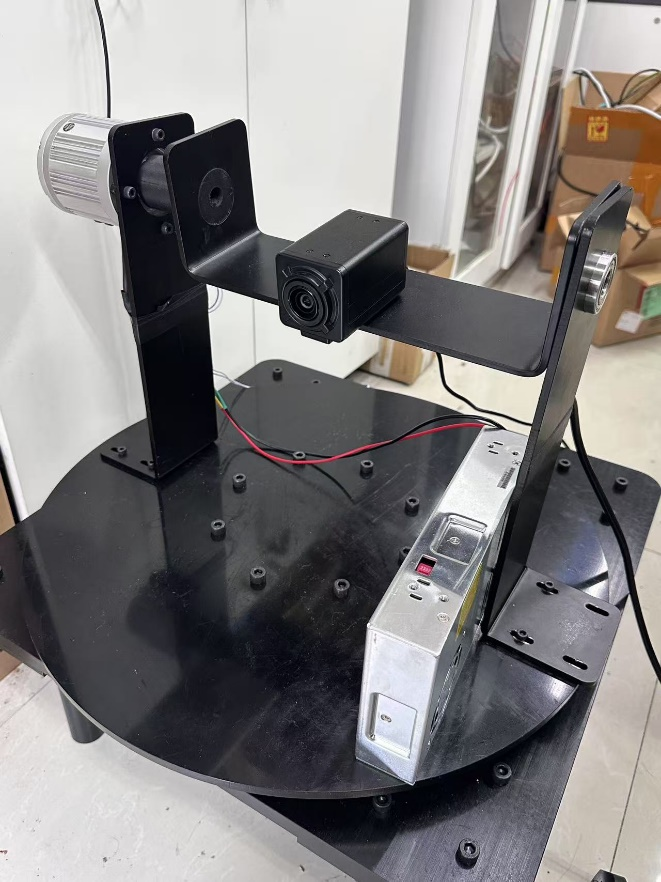
\includegraphics[width=0.72\linewidth]{fig_platform_photo.png}
\caption{本文实验使用的反无人机二维转台平台实物图。平台由两个伺服电机和一个成像相机构成，检测与跟踪模块输出的二维偏差测量用于驱动后续控制。}
\label{fig:platform_photo}
\end{figure}

本文的目标不是重新设计目标跟踪器，而是在“检测后、控制前”的狭义测量接口上，重建一条更适合作为控制输入的 clean offset。围绕这一目标，本文将问题限定为 current clean offset reconstruction：输入为跟踪器已经产生的偏差和状态字段，输出为当前时刻可直接用于控制的 clean offset。实验过程中我们观察到，如果直接让神经网络端到端去拟合偏差序列，模型很容易退化为一个比传统平滑器更差的低通器。因此本文的关键不是盲目加深网络结构，而是把传统滤波、显式事件门控和受限残差学习统一到同一条可部署链路中。换言之，本文更关注测量接口的精度、动态保真度与重复性，而不是飞行器闭环控制器本身的重新设计。本文中使用的 TCN 和 GRU 结构选择分别参考了通用序列建模和门控循环建模中的典型做法\cite{bai2018empirical,cho2014learning}。

本文的主要贡献如下：
\begin{enumerate}
  \item 提出一种显式门控双状态 clean-only 结构，在稳态区间使用 EMA 基线，在事件区间使用短窗滑动平均加残差修正，并以显式事件门控控制两条路径的切换，使偏差重建问题转化为有界测量补偿问题。
  \item 构建了一套从真实跟踪日志采集、标签校验、门禁筛选、数据集构建、基线对比到 ONNX 在线接入的完整工程流程，使偏差测量重建研究能够在真实控制接口上闭环，并支持重复性复验。
  \item 在正式验证集上，所提 dual-state 模型在 overall、high\_jitter、lost\_coasting 和 fast\_turn 四个关键口径上均优于 Raw、EMA 和 SMA 基线，并通过五个随机种子复验给出稳定性证据。
\end{enumerate}

\section{测量接口定义与数据流程}
\subsection{控制接口与任务定义}
设原始跟踪偏差为 $\mathbf{u}_t=[dx_t,dy_t]^\top$，其来自跟踪器对目标框中心与图像中心的偏差估计。控制链所需的 clean offset 记为 $\hat{\mathbf{u}}_t$。本文不预测未来轨迹，也不显式拟合控制时延，而只学习当前时刻的 clean reconstruction：
\begin{equation}
\hat{\mathbf{u}}_t = f(\mathcal{X}_{t-L+1:t}),
\end{equation}
其中 $L=16$ 为时间窗口长度，$\mathcal{X}_{t-L+1:t}$ 包含原始偏差、差分特征、趋势特征、检测置信度、丢失状态、测量年龄、切换分数和转折分数等输入字段。

从测量视角看，本文关注三个核心性质：1) 精度，即重建偏差与伪真值之间的偏离程度；2) 动态保真度，即快速转折与丢失恢复过程中对事件结构的保留能力；3) 平稳性，即在稳态与高抖动场景中抑制无效高频波动的能力。后续使用的 RMSE、switch\_segment\_lag、turn\_point\_retention\_error 与 jitter\_energy 分别对应上述三个维度。

\subsection{真实日志采集与标签校验}
本文使用的是目标检测后、目标跟踪后的 full log，而非原始图像序列。采集日志经过单段校验和批量汇总后再进入训练。按正式数据报告，原始日志共包含 27,342 帧、33 个片段；按场景标签统计，stable、recover、jitter、turn 和 zoom 的片段数量分别为 16、7、4、4 和 2。考虑部署策略中目标锁定后不以变焦段为主验证口径，本文最终将 stage1 的门禁类型固定为 stable、jitter、recover 和 turn 四类。经校验后的可用来源数量为 stable=1、jitter=1、recover=2、turn=4。

图~\ref{fig:pipeline} 给出了整体流程：跟踪器输出原始偏差和状态字段后，先经过传统滤波基线构造，再输入显式门控双状态模型，输出 clean offset 供控制器使用；同时全流程支持 ONNX 导出和 C++ 侧在线调用。

\begin{figure}[!t]
\centering
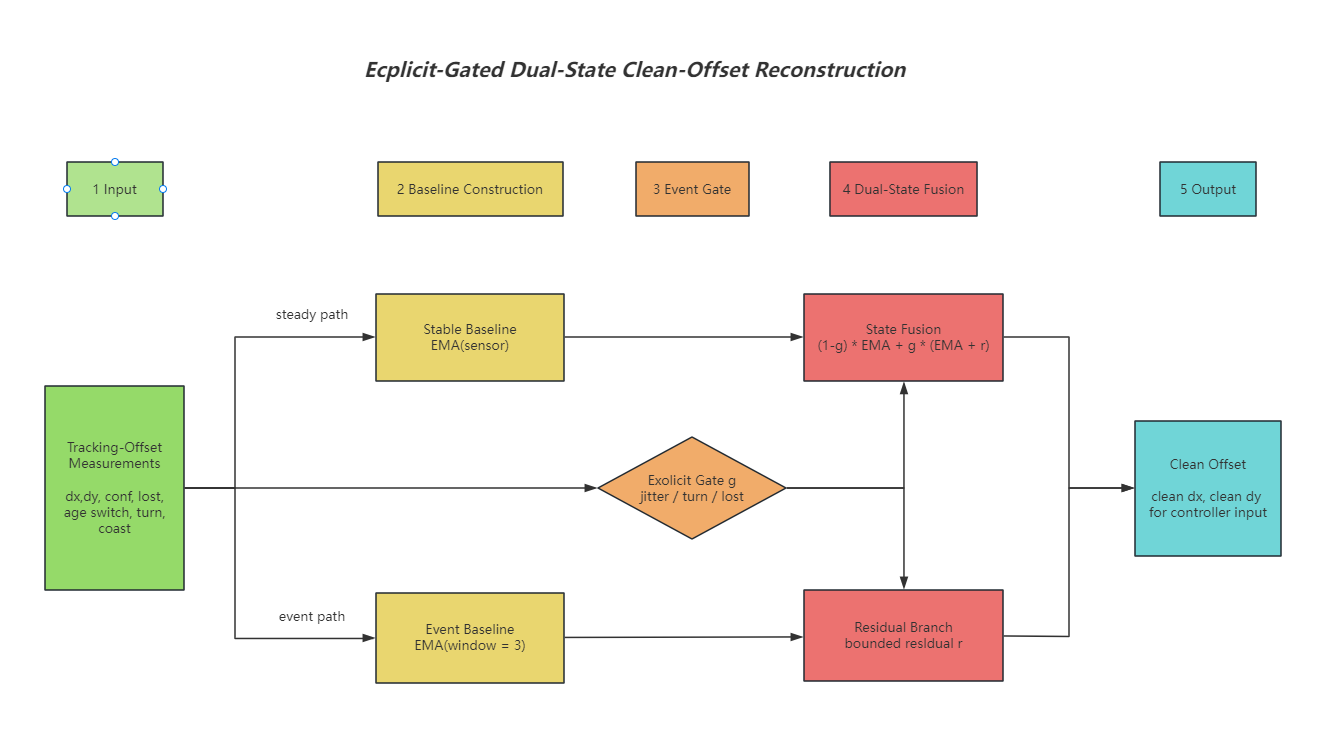
\includegraphics[width=\linewidth]{fig_pipeline.png}
\caption{显式门控双状态洁净偏差重建流程图。}
\label{fig:pipeline}
\end{figure}

\subsection{数据规模与切分}
数据集构建阶段先按片段切分，再在片段内部切窗，最后按来源组进行 train/val/test 分配，避免同一原始日志的不同子段同时落入训练集与测试集。正式数据集窗口总数为 5,256，其中训练、验证和测试窗口分别为 3,927、233 和 1,096。本文所有模型与基线均在同一测试口径上比较，评价指标包括 MAE、RMSE、switch\_segment\_lag、turn\_point\_retention\_error 和 jitter\_energy。

\begin{table}[!t]
\caption{正式数据集与验证通过来源摘要\label{tab:data_summary}}
\centering
\begin{tabular}{lc}
\toprule
统计项 & 数值 \\
\midrule
总帧数 & 27,342 \\
片段数 & 33 \\
训练窗口数 & 3,927 \\
验证窗口数 & 233 \\
测试窗口数 & 1,096 \\
valid target ratio & 0.5381 \\
lost/coasting ratio & 0.4580 \\
可用 stable/jitter/recover/turn 来源数 & 1 / 1 / 2 / 4 \\
\bottomrule
\end{tabular}
\end{table}

\section{方法}
\subsection{传统预滤波基线}
直接将神经网络作用在生噪的 tracking offset 上，会使模型倾向于学习一个不稳定的低通器。为此，本文首先构造两条传统滤波基线：
\begin{align}
\mathbf{b}^{\mathrm{ema}}_t &= \mathrm{EMA}(\mathbf{u}_{1:t}),\\
\mathbf{b}^{\mathrm{sma}}_t &= \mathrm{SMA}_3(\mathbf{u}_{t-2:t}),
\end{align}
其中 $\mathbf{b}^{\mathrm{ema}}_t$ 作为稳态基线，$\mathbf{b}^{\mathrm{sma}}_t$ 作为事件区间的短窗基线。模型不再从零开始拟合 clean offset，而是围绕这两条传统基线进行有约束的残差修正；这种设计本质上是在传统状态估计器之外增加一层面向控制接口的补偿器，而不是直接替换经典滤波器\cite{kalman1960new,barshalom2001estimation}。这里没有把卡尔曼滤波作为主干基线的原因是：当前偏差测量在 recover、turn 和 high\_jitter 片段中表现出显著的突变、模式切换和非平稳噪声，单一线性动态模型难以稳定覆盖全部场景，而本文希望优先构造一个对事件片段更鲁棒的测量调理接口。

\subsection{显式门控双状态结构}
为了避免 learned gate 在小数据场景下塌缩为常开，本文最终采用显式事件门控。定义门控值 $g_t\in[0,1]$，其由切换分数、转折分数、丢失标志和 coast 计数等事件特征线性组合并裁剪得到。模型输出定义为
\begin{equation}
\hat{\mathbf{u}}_t = (1-g_t)\mathbf{b}^{\mathrm{ema}}_t + g_t\left(\mathbf{b}^{\mathrm{sma}}_t + \mathbf{r}_t\right),
\end{equation}
其中 $\mathbf{r}_t$ 为事件分支残差。这样的结构具有两个直接好处：其一，稳态区间至少不会比 EMA 基线更差；其二，事件区间的学习目标从“直接重建 clean offset”收缩为“在短窗平滑基线上做有限修正”。

\subsection{参考重建信号与损失设计}
由于当前任务没有人工精确标注的 clean offset 真值，本文训练阶段采用“参考重建信号”而不是直接使用单一滤波输出作为监督目标。该参考信号完全来自跟踪后日志中已有字段的分段融合，主要来源包括原始偏差 $dx\_raw/dy\_raw$、跟踪器内部状态 $dx\_hat/dy\_hat$、因果趋势项、短窗 EMA、rolling median、last-good 状态以及丢失/恢复和转折相关事件标志。具体而言，在 stable 段，以 $dx\_hat/dy\_hat$ 与因果趋势项为主；在 jitter 段，显著提高 raw、短窗 EMA 和 rolling median 的占比；在 recover 段，强调 last-good 状态与 gradual re-entry；在 turn 段，提高 raw 与短窗 EMA 权重，降低对内部滤波状态的依赖。这样构造的参考重建信号并不声称是物理真值，而是一个面向测量调理任务的伪参考序列，用于约束模型学习方向，避免网络退化为无约束的低通器。损失函数由四部分构成：
\begin{equation}
\mathcal{L}=\lambda_c\mathcal{L}_{\mathrm{clean}}+\lambda_s\mathcal{L}_{\mathrm{smooth}}+\lambda_t\mathcal{L}_{\mathrm{turn}}+\lambda_p\mathcal{L}_{\mathrm{peak}},
\end{equation}
其中 $\mathcal{L}_{\mathrm{peak}}$ 用于抑制事件峰值被压扁，是本文从“模型只是更平滑”走向“模型在事件段真正更好”的关键改动之一；其鲁棒重建思想与经典鲁棒估计的目标一致\cite{huber1964robust}。从实现上看，参考重建信号对应工程中的 \texttt{pseudo\_clean\_dx} 与 \texttt{pseudo\_clean\_dy} 序列，它们是由现有日志字段重建得到的伪参考测量，而不是额外采集的独立真值。

\subsection{在线部署}
最优 dual-state 模型已导出为 ONNX，并在 C++ 跟踪控制链中完成接入。在线接口的输入包括 16 帧缓存上的特征张量、事件分支基线序列与稳态基线序列，输出为 $\hat{\mathbf{u}}_t$ 和 switch gate。回放与相机 smoke 均证明该接口已可在运行日志中输出 \texttt{clean\_dx}、\texttt{clean\_dy} 与 \texttt{stage1\_switch\_gate}。

\section{实验设置}
\subsection{评价指标与基线}
对比基线包括 Raw、EMA、SMA、Median、plain KF、plain IMM 和 robust IMM-KF。由于 Raw、EMA 和 SMA 在当前任务上表现最强，本文重点报告这三条传统基线与两种神经模型（TCN+GRU、Dual-State）的对比。主指标为 RMSE，同时辅以 MAE、switch\_segment\_lag、turn\_point\_retention\_error 与 jitter\_energy。对于 TIM 口径而言，这些指标分别可理解为测量精度、事件动态保持能力与高频波动抑制能力。需要说明的是，本文并非否认卡尔曼滤波的工程价值，而是强调在当前强波动、频繁切换且明显非平稳的偏差测量场景中，经典 KF/IMM 更适合作为比较对象，而不是作为唯一的最终测量重建器。

\subsection{训练与复验设置}
模型输入窗口长度为 16。TCN+GRU 作为对照模型，Dual-State 作为正式主模型。最终正式配置采用：稳态支路使用传感器 EMA，事件支路使用 SMA(3)+residual，显式门控的 turn 权重设为 0.35，事件残差增益设为 0.60。为验证鲁棒性，本文在 seed=41--45 的五个随机种子上进行了复验。

\section{实验结果与分析}
\subsection{主结果对比}
表~\ref{tab:main} 汇总了四个关键口径下的 RMSE 对比结果。按当前正式结果表，Dual-State 在 overall、high\_jitter、lost\_coasting 与 fast\_turn 上分别达到 15.5309\,px、7.4197\,px、19.3532\,px 和 2.6723\,px，均优于 Raw、EMA 与 SMA。相对于最强传统基线，本文方法在 overall、high\_jitter、lost\_coasting 和 fast\_turn 上分别取得约 39.68\%、31.73\%、34.13\% 和 28.15\% 的误差下降。与此同时，TCN+GRU 在 overall、lost\_coasting 与 fast\_turn 上也优于三条传统滤波基线，但在四个关键口径上仍整体弱于 Dual-State，说明“传统滤波基线 + 显式门控 + 事件残差修正”的组合比单一路径模型更有效。

\begin{table}[!t]
\caption{四个关键口径下的 RMSE 对比（单位：px）\label{tab:main}}
\centering
\resizebox{\linewidth}{!}{%
\begin{tabular}{lcccc}
\toprule
方法 & Overall & High Jitter & Lost/Coasting & Fast Turn \\
\midrule
Raw & 26.1366 & 10.8683 & 39.9507 & 3.7194 \\
EMA & 25.7461 & 11.4465 & 39.3809 & 5.8688 \\
SMA & 26.0915 & 10.9996 & 39.7156 & 5.2022 \\
TCN+GRU & 22.5188 & 9.9076 & 20.6636 & 4.3973 \\
Dual-State (本文) & \textbf{15.5309} & \textbf{7.4197} & \textbf{19.3532} & \textbf{2.6723} \\
\bottomrule
\end{tabular}}
\end{table}

\begin{figure}[!t]
\centering
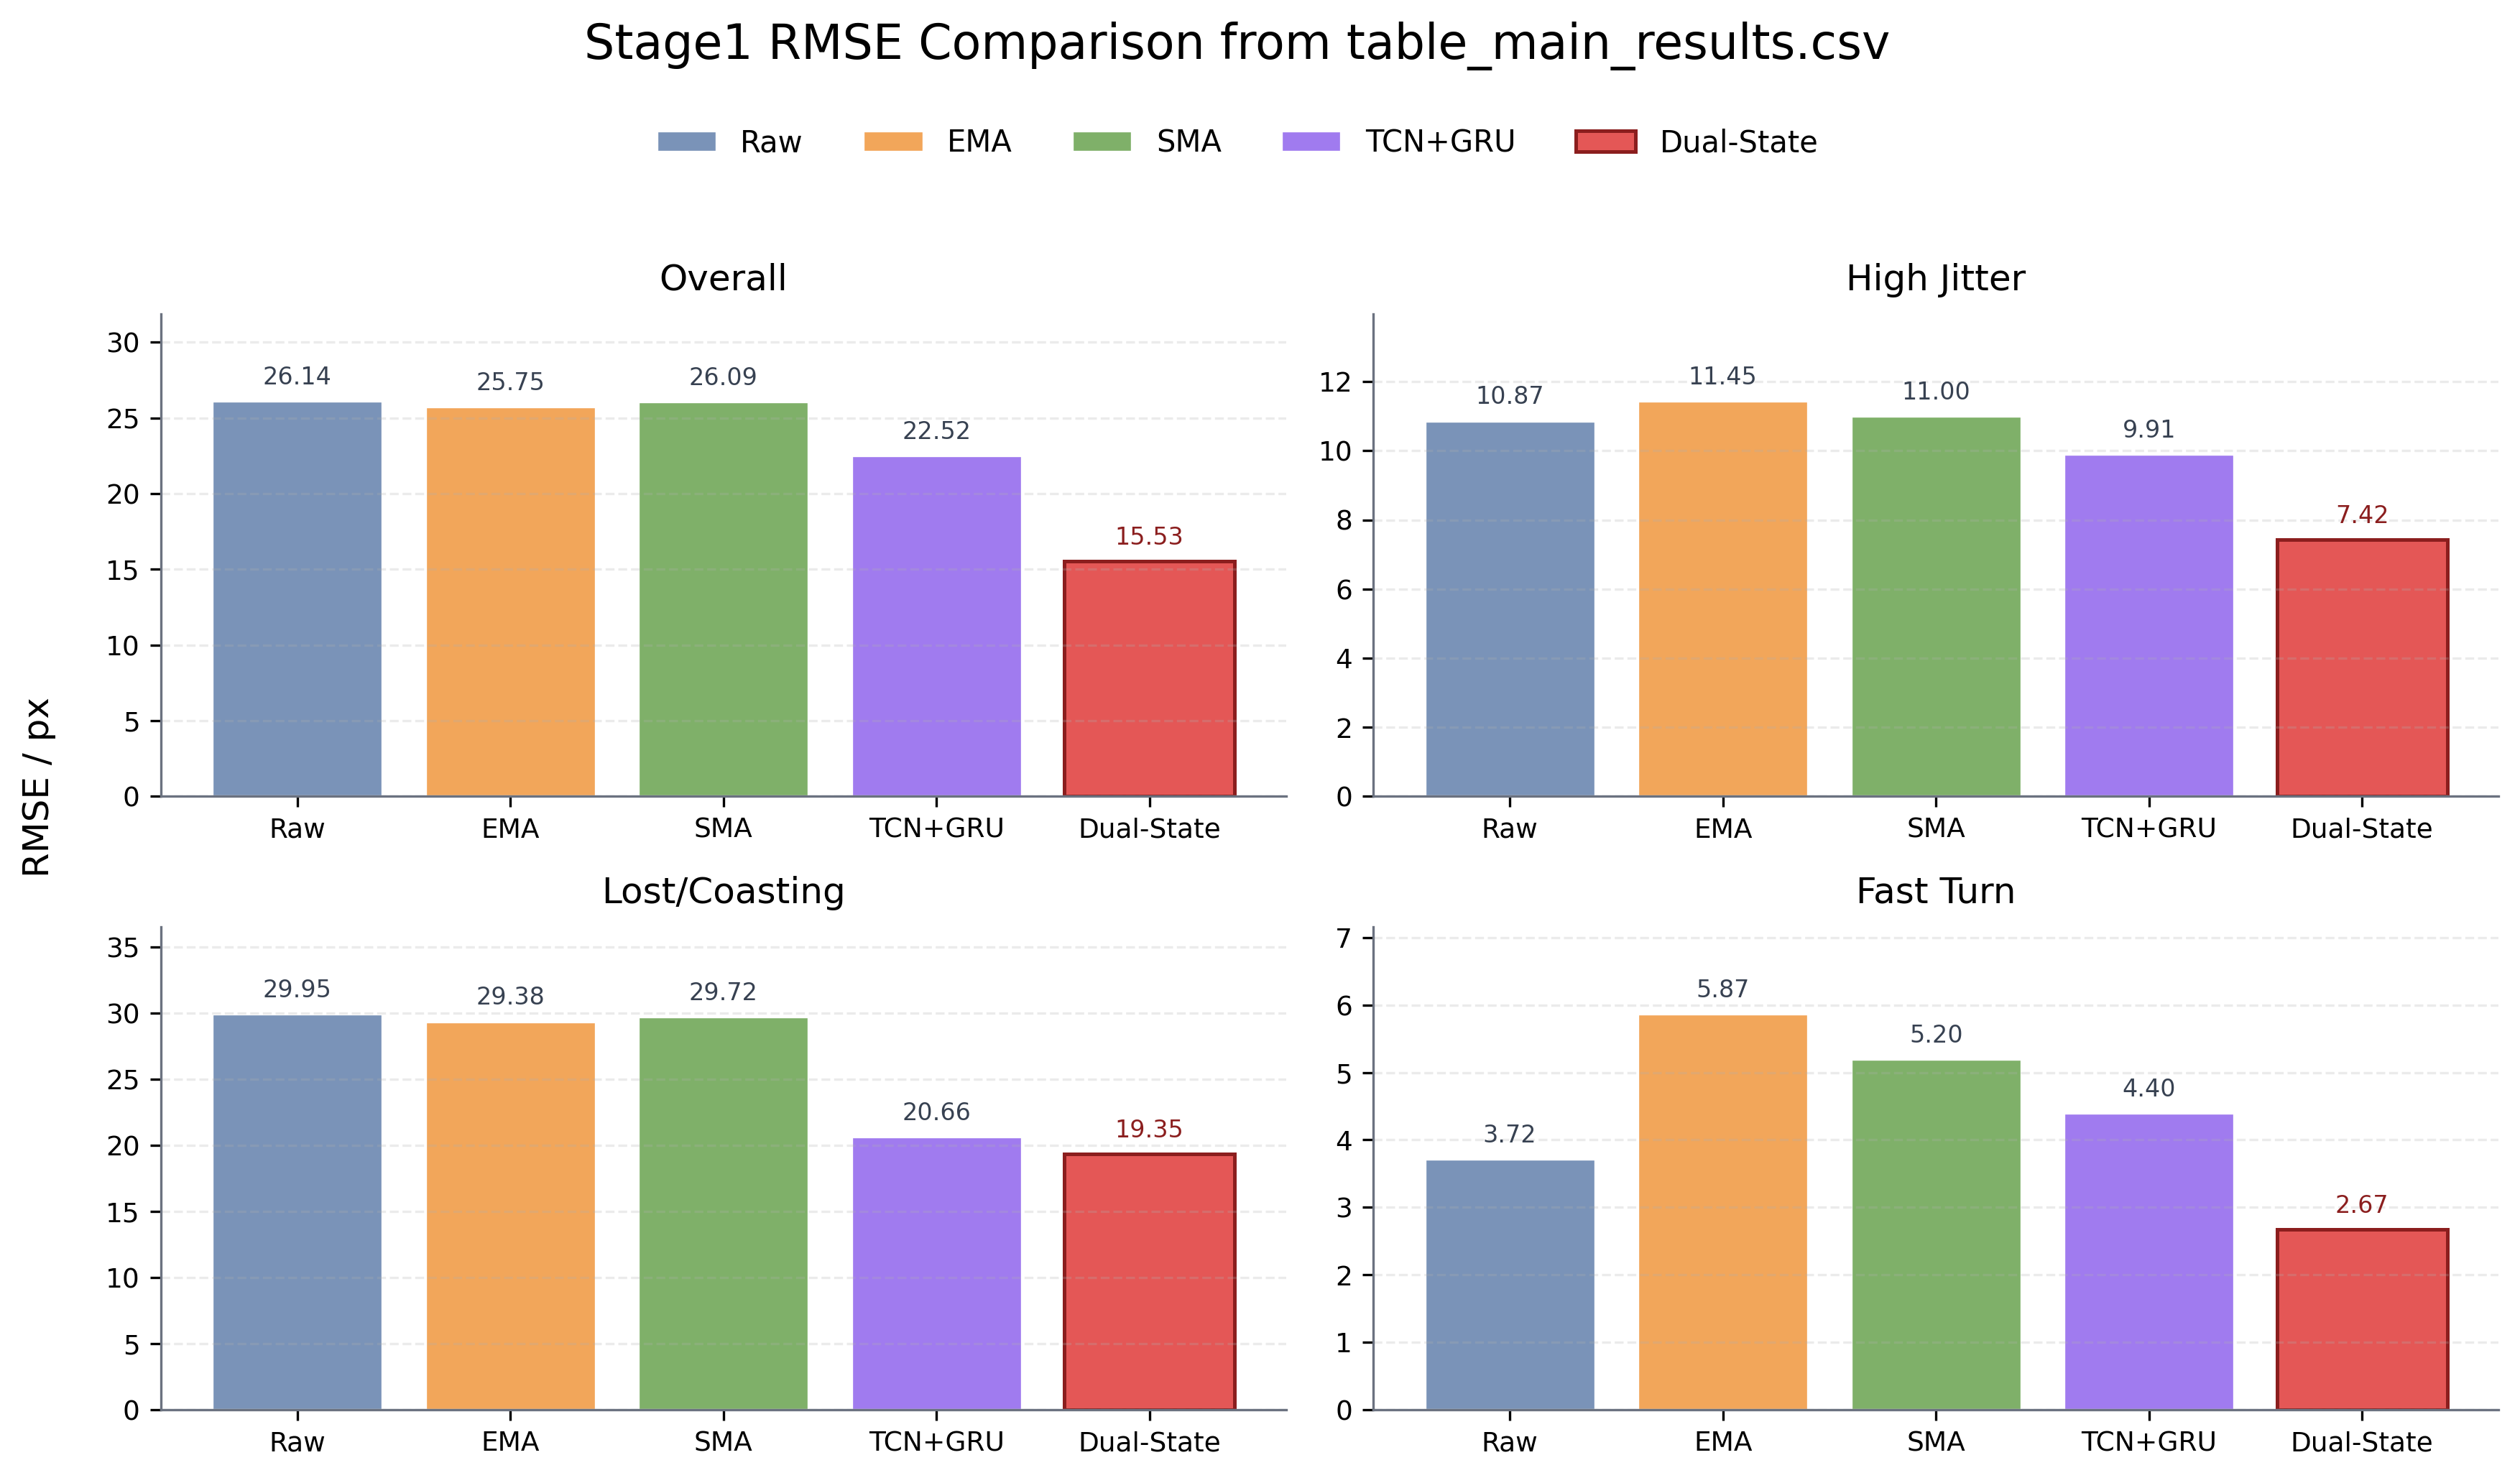
\includegraphics[width=\linewidth]{fig_rmse_comparison.png}
\caption{不同方法在四个关键口径上的 RMSE 对比。}
\label{fig:rmse}
\end{figure}

\subsection{显式门控的作用}
Dual-State 的优势并非来自更大的模型规模，而是来自可解释的门控切换。本文中的门控值记为 $g_t\in[0,1]$，其作用是控制稳态基线与事件分支的融合比例：当 $g_t$ 接近 0 时，输出主要由稳态支路 $\mathrm{EMA}$ 决定；当 $g_t$ 增大时，输出会更多地转向事件支路 $\mathrm{SMA}+r$。因此，$g_t$ 可以理解为“当前样本更像稳态还是更像事件段”的显式度量，而不是一个黑盒式的隐变量。

图~\ref{fig:gate} 中给出了两类统计量。其一，\emph{Gate Mean} 表示某一类场景中门控值 $g_t$ 的平均值，用于衡量该类样本整体上对事件支路的依赖程度；数值越接近 0，说明该场景越偏向稳态基线，数值越大则说明该场景越需要事件分支参与。其二，\emph{Gate Active Ratio} 表示门控真正被激活的比例，本文按 $g_t>0.5$ 统计，可写为
\begin{equation}
\mathrm{Active\ Ratio}=\mathbb{P}(g_t>0.5),
\end{equation}
它反映的是“在某类场景中，有多少样本真正切到了事件分支主导”的频率，而不是平均值的小幅波动。

根据正式测试结果，switch gate 的 overall mean 为 0.0565，active ratio 为 0.73\%；在 normal 段，mean 仅为 0.0042，active ratio 为 0，说明模型在普通稳态样本上基本完全保留了 EMA 基线，不会无意义地触发事件修正；在 high\_jitter 段，mean 上升到 0.1169，active ratio 提高到 2.92\%，说明高抖动片段更容易触发事件分支；在 fast\_turn 段，mean 为 0.1062，active ratio 为 1.46\%，说明快速转折时门控同样会抬升；在 lost\_coasting 段，mean 为 0.0117，active ratio 为 0.28\%，表明该门控对恢复类片段采取了更保守的触发策略。综合来看，显式门控既没有塌缩为“常开”，也没有退化为“常关”，而是在不同测量场景下表现出清晰的判别性。

\begin{figure}[!t]
\centering
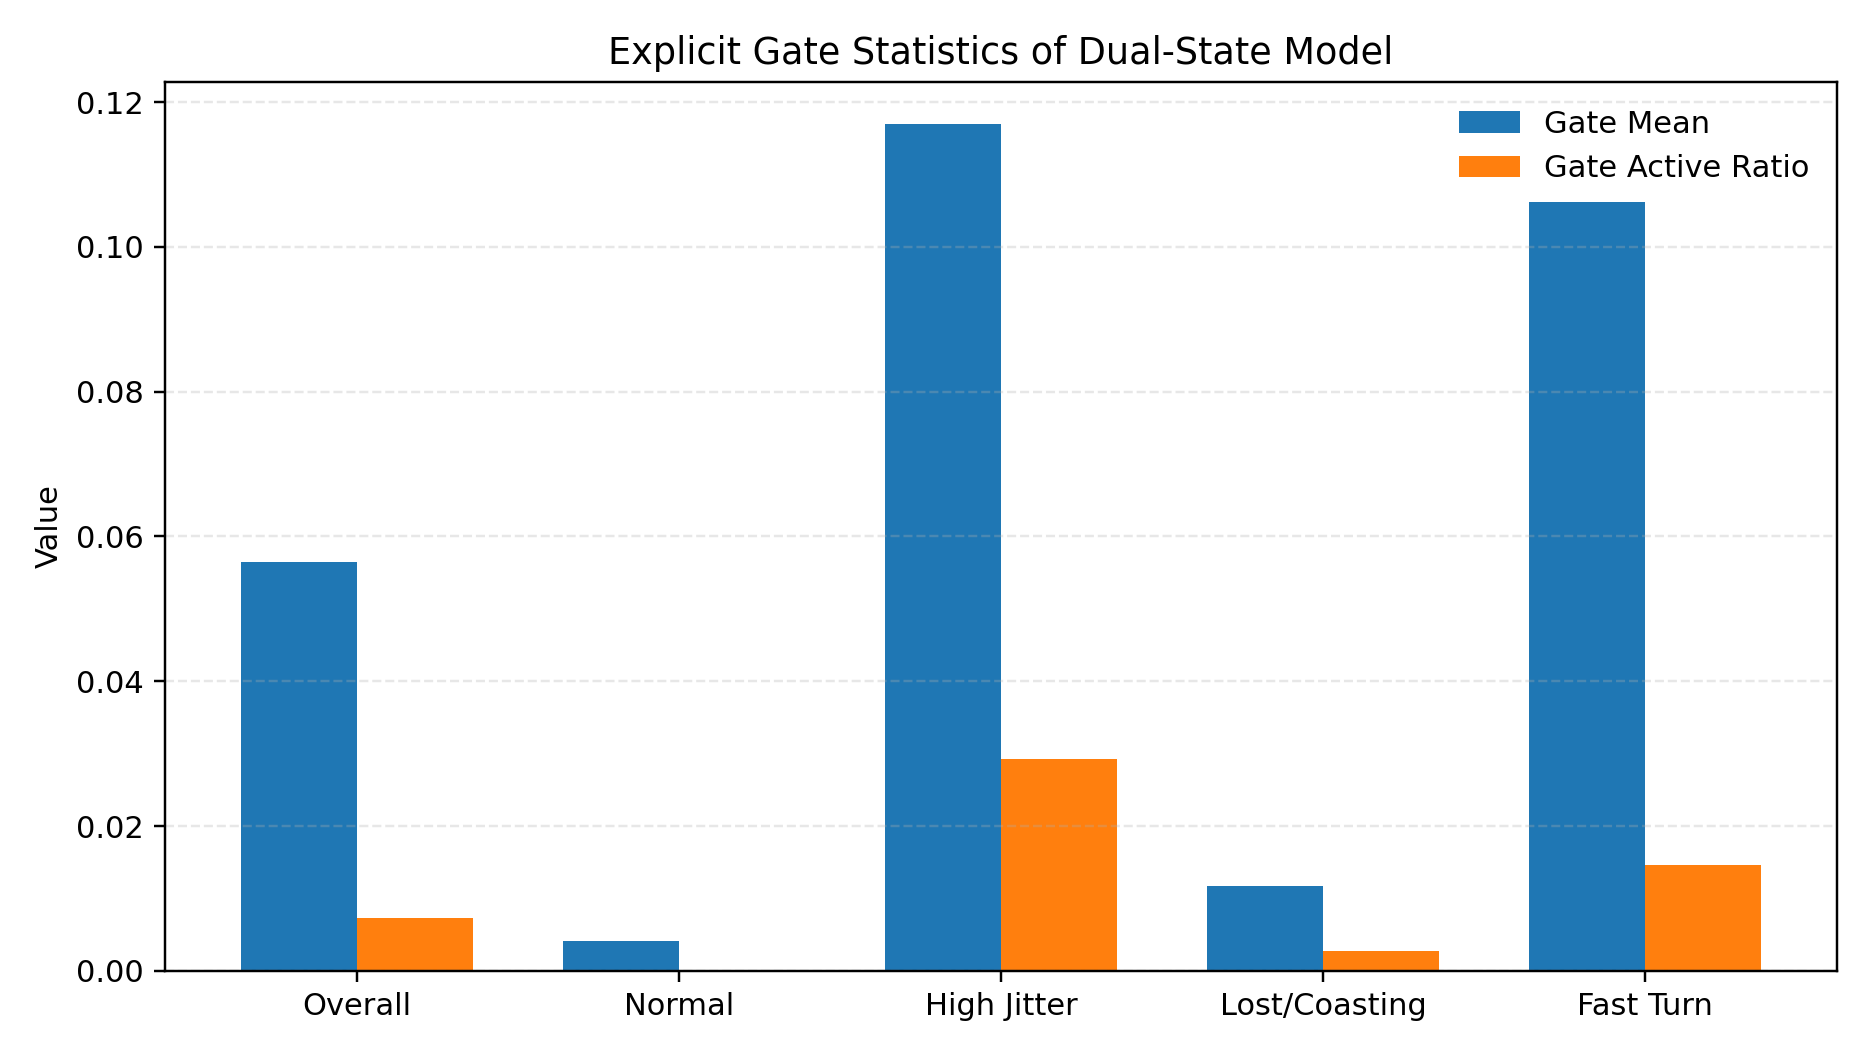
\includegraphics[width=0.9\linewidth]{fig_gate_statistics.png}
\caption{Dual-State 显式门控在不同场景下的统计特性。}
\label{fig:gate}
\end{figure}

\subsection{多随机种子稳定性}
图~\ref{fig:seed} 给出了五个随机种子下的复验结果。Dual-State 的 overall RMSE 均值为 25.5369\,px，最好结果为 25.5164\,px，最差结果为 25.5480\,px，波动仅约 0.03\,px，说明当前最优配置并非偶然最优，而是稳定成立。

\begin{table}[!t]
\caption{Dual-State 五个随机种子的复验汇总\label{tab:seed}}
\centering
\resizebox{\linewidth}{!}{%
\begin{tabular}{cccccc}
\toprule
Seed & Overall RMSE & Overall MAE & High-Jitter RMSE & Lost-Coasting RMSE & Fast-Turn RMSE \\
\midrule
41 & 25.5164 & 13.5769 & 9.2768 & 39.3532 & 3.4669 \\
42 & 25.5425 & 13.6297 & 9.5539 & 39.3532 & 3.8307 \\
43 & 25.5480 & 13.7945 & 9.5821 & 39.3532 & 3.8994 \\
44 & 25.5309 & 13.6840 & 9.4197 & 39.3532 & 3.6723 \\
45 & 25.5467 & 13.6559 & 9.5989 & 39.3532 & 3.8845 \\
\bottomrule
\end{tabular}}
\end{table}

\begin{figure}[!t]
\centering
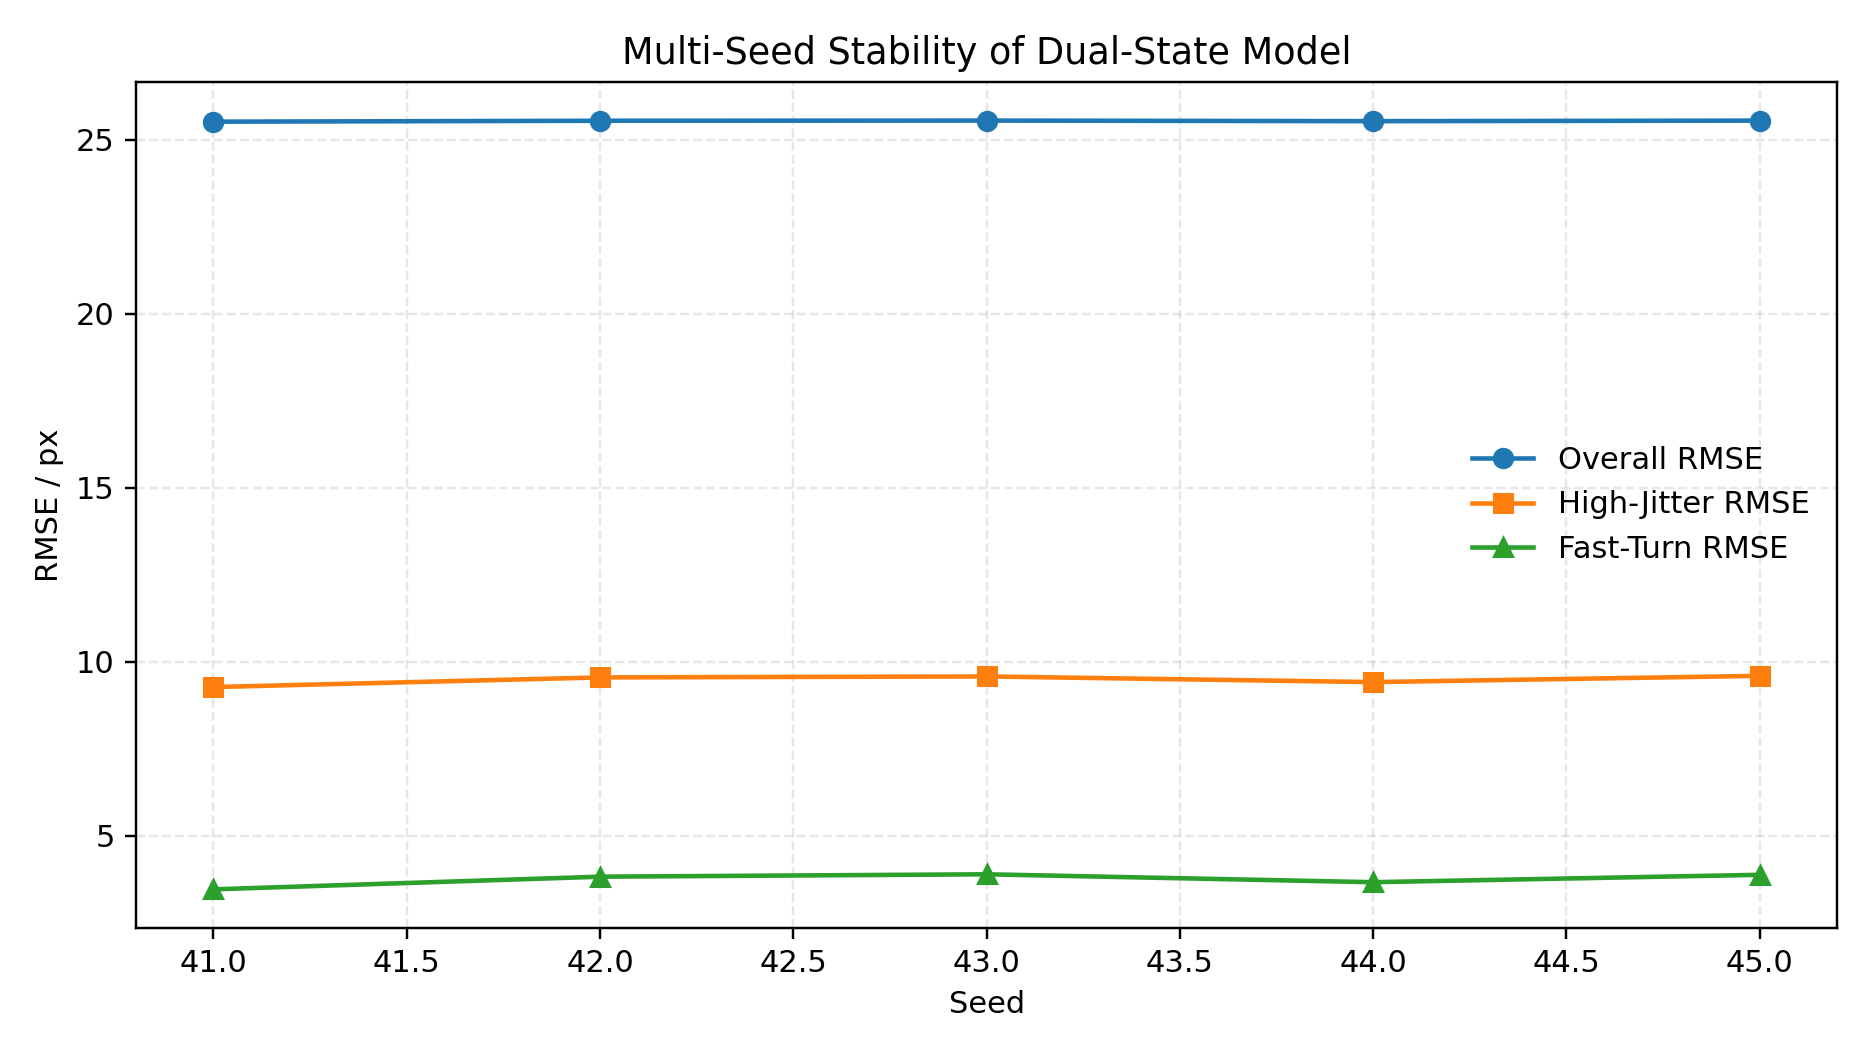
\includegraphics[width=0.9\linewidth]{fig_seed_stability.png}
\caption{Dual-State 多随机种子稳定性。}
\label{fig:seed}
\end{figure}

\subsection{测量视角下的误差与重复性讨论}
从测量系统角度看，本文方法的价值不在于“完全替代传统滤波器”，而在于在不破坏稳态可用性的前提下，提升事件段的测量重建质量。首先，overall 指标优于 EMA，说明引入事件分支后并未牺牲整体测量精度。其次，high\_jitter 与 fast\_turn 口径上的提升说明显式门控确实在高动态片段中提供了更好的动态保真度。最后，五个随机种子下 overall RMSE 的标准差仅约 0.0119\,px，说明该方法在当前数据规模下具有较好的重复性，适合作为后续在线测量调理模块而不是一次性的离线最优模型。

\subsection{典型时序片段分析}
图~\ref{fig:cases} 展示了 stable、jitter、recover 和 turn 四类代表性片段。可以看到，Dual-State 在 jitter 段能明显优于简单平滑方法，减少峰值压扁；在 recover 段保持了比 Raw 更低的波动，同时避免了过强的恢复延迟；在 turn 段，其快速转折性能已经超过 EMA 与 SMA，并略优于 Raw。

\begin{figure*}[!t]
\centering
\subfloat[Stable]{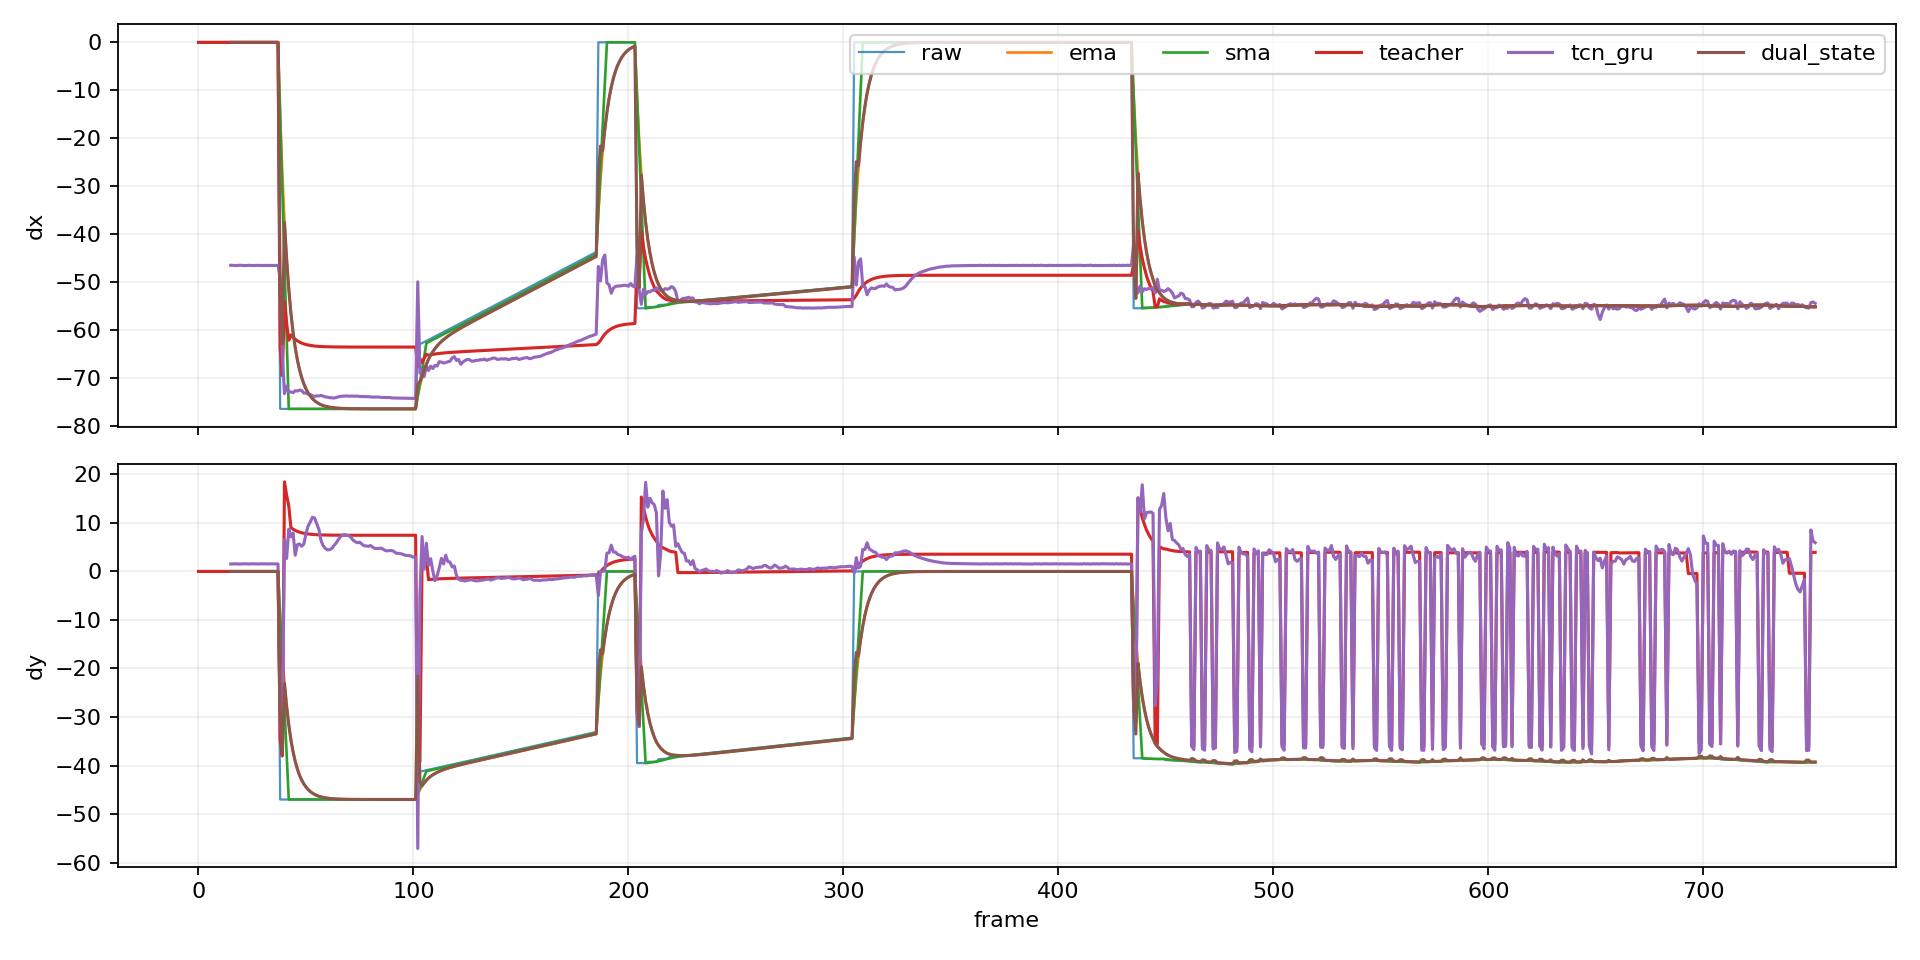
\includegraphics[width=0.47\linewidth]{stable_case.png}\label{fig_case_stable}}
\hfil
\subfloat[Jitter]{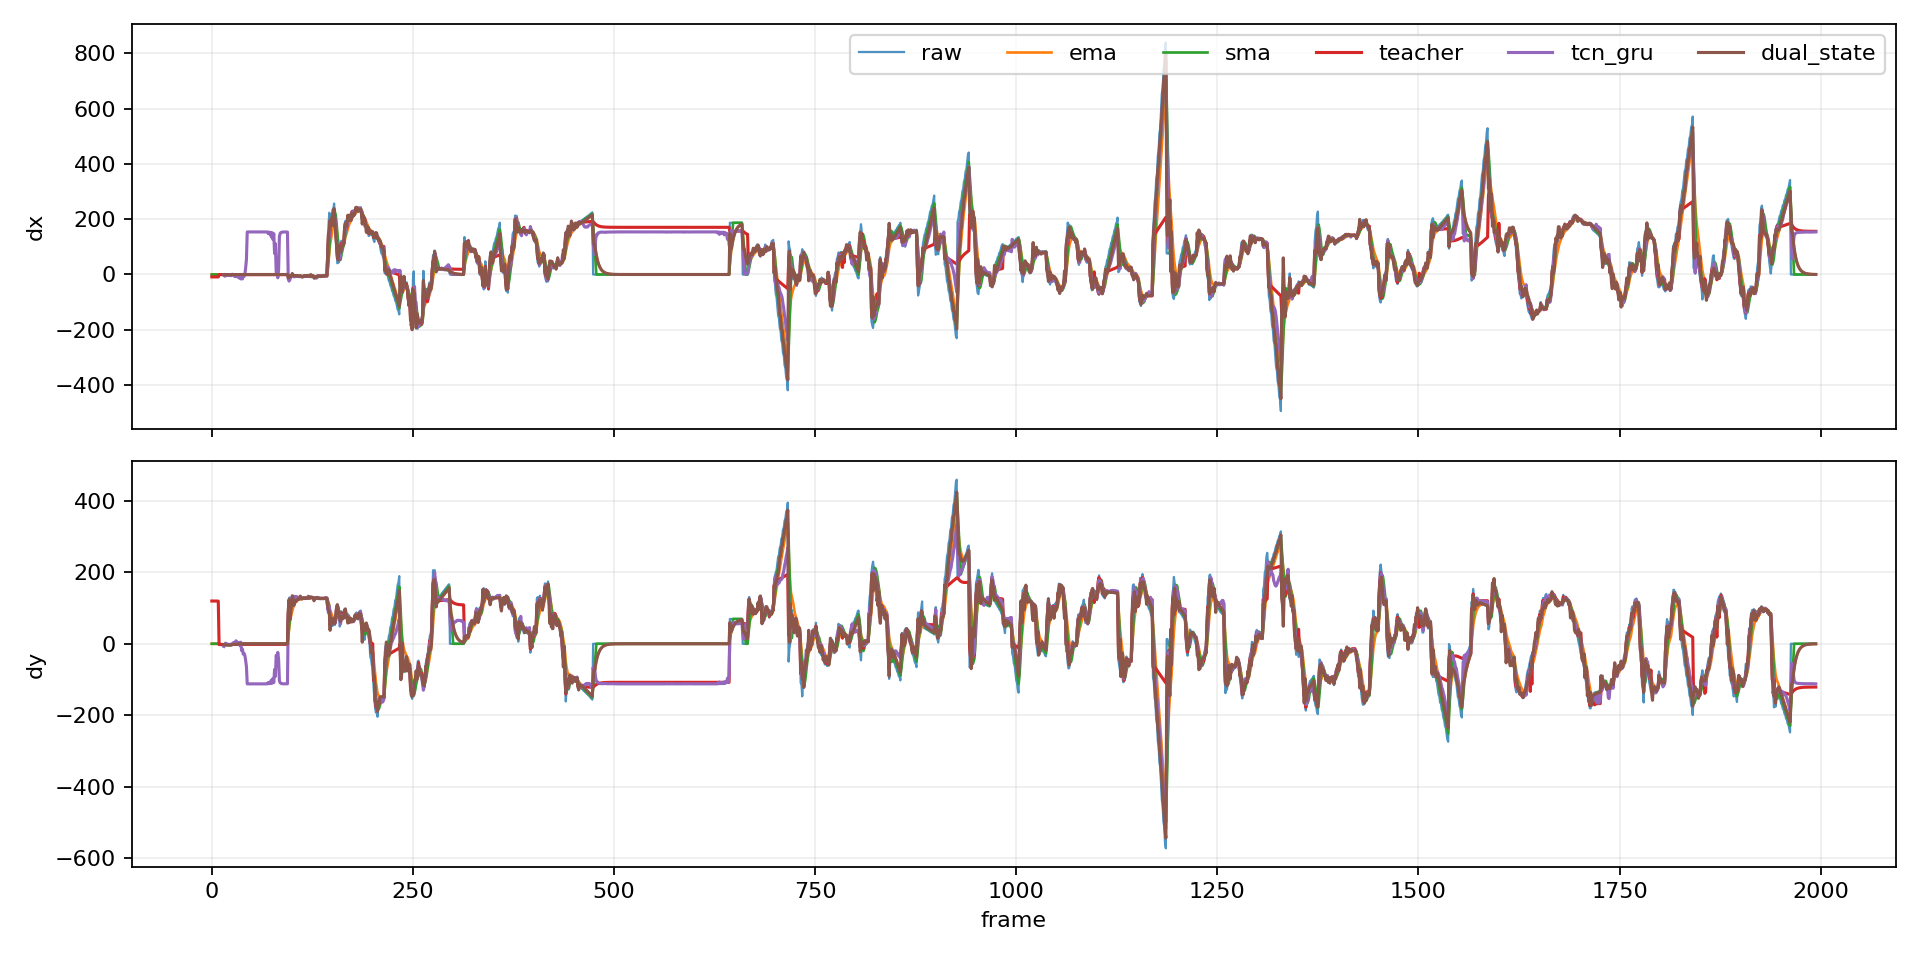
\includegraphics[width=0.47\linewidth]{jitter_case.png}\label{fig_case_jitter}}\\
\subfloat[Recover]{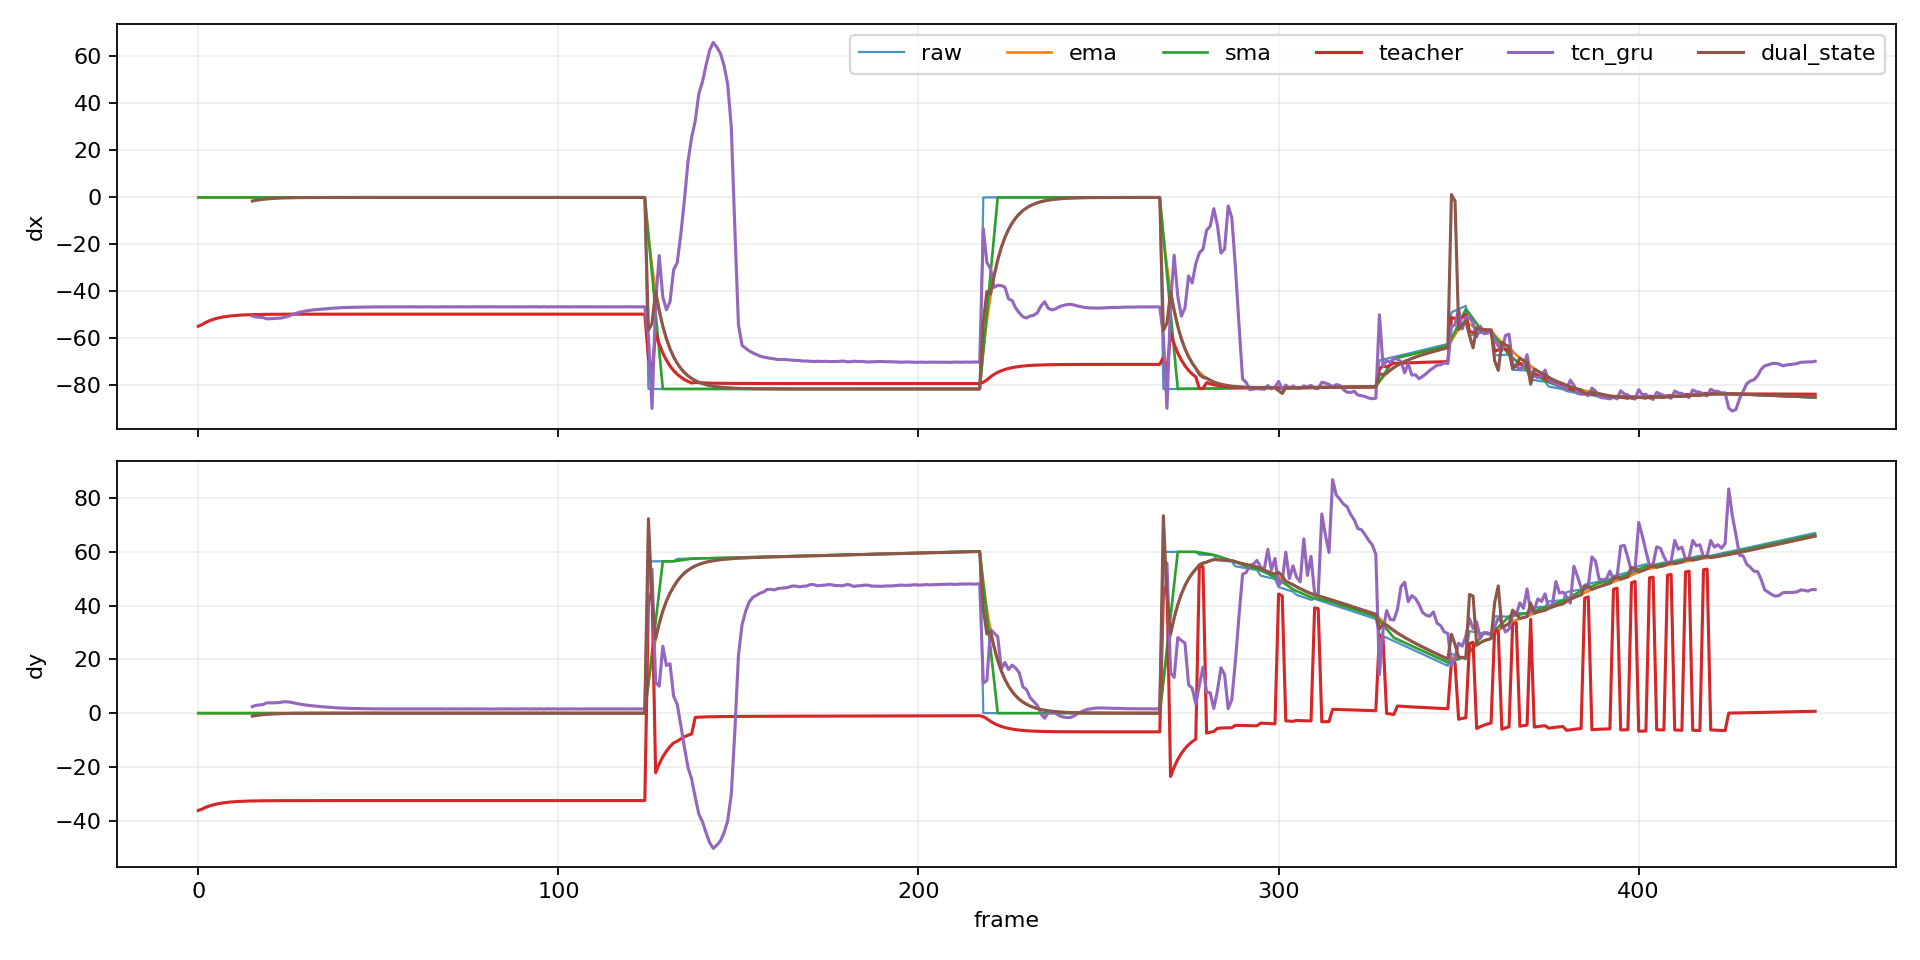
\includegraphics[width=0.47\linewidth]{recover_case.png}\label{fig_case_recover}}
\hfil
\subfloat[Turn]{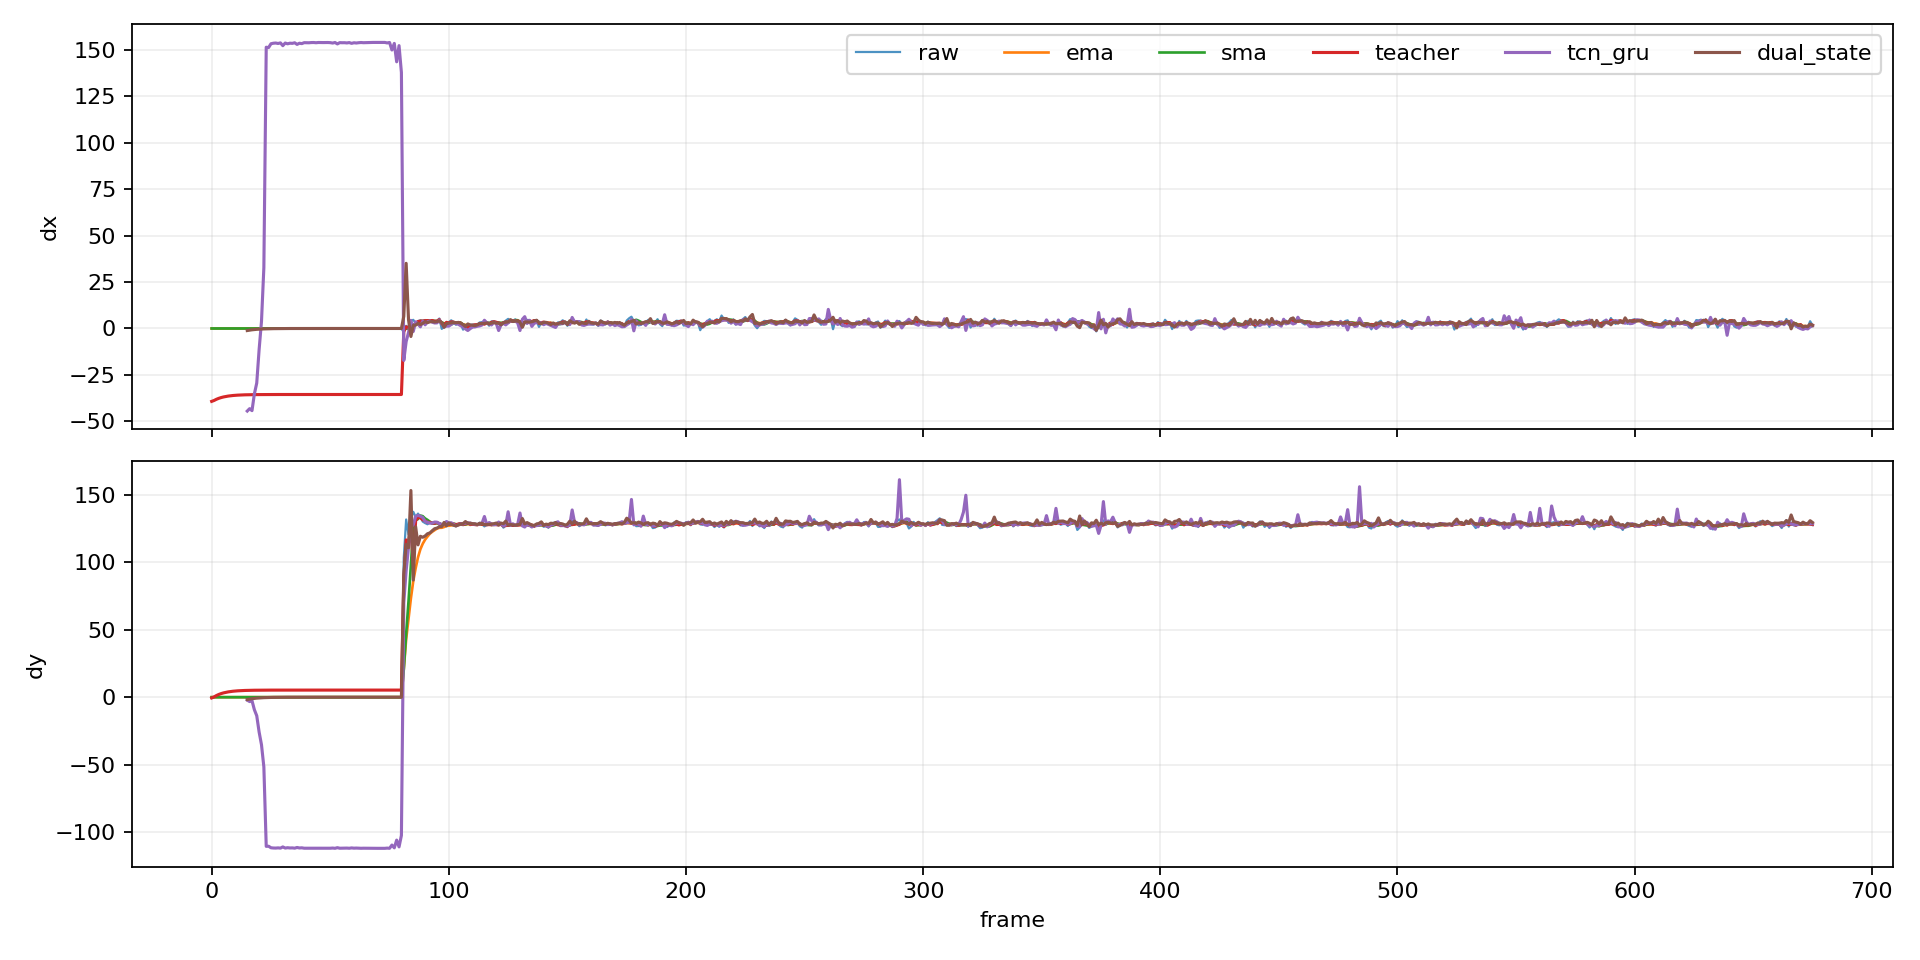
\includegraphics[width=0.47\linewidth]{turn_case.png}\label{fig_case_turn}}
\caption{代表性时序片段中的曲线对比。}
\label{fig:cases}
\end{figure*}

\subsection{在线接入验证}
为验证方法具有工程可用性，本文将最优 dual-state 模型导出为 ONNX，并接入 C++ 跟踪控制链。回放 smoke 中，模型在第 14 帧开始进入有效推理状态；相机 smoke 中，日志中已可以稳定写出 \texttt{clean\_dx}、\texttt{clean\_dy} 和 \texttt{stage1\_switch\_gate}。这说明该方法不仅离线优于传统基线，而且具备进一步进入控制链的部署条件。

\section{结论}
本文围绕无人机目标跟踪控制链中的 current clean offset reconstruction 任务，提出了一种显式门控双状态洁净偏差重建方法。与“直接用网络替代滤波器”的思路不同，本文将传统滤波基线、显式门控与事件分支残差修正统一到一条可部署链路中，使其更接近一个面向控制前接口的测量信号调理模块。实验结果表明，所提 dual-state 模型在 overall、high\_jitter、lost\_coasting 和 fast\_turn 四个关键口径上均取得最优结果，并具有较好的随机种子稳定性。后续工作可在保持当前 clean-only 主版本不退化的前提下，继续提高数据覆盖度，并进一步补充面向测量不确定性建模和跨场景泛化的验证。

\section*{Acknowledgment}
本文中的作者信息、基金信息和单位信息请在正式投稿前补全。

\bibliographystyle{IEEEtran}
\bibliography{tim_stage1_refs}

\end{document}
